\documentclass[12pt]{report}

% Packages
\usepackage{graphicx}     % For images
\usepackage{fancyhdr}     % For headers and footers
\usepackage[top=2.5cm, left=2.5cm, right=2.5cm, bottom=2.5cm, headheight=1.25cm, footskip=1.25cm]{geometry} % Page Margins
\usepackage{iflang}       % For language conditional commands
\usepackage{polyglossia}  % For multiple languages
\usepackage{fontspec}     % For specifying fonts


%=================================================================
% Language settings, swith the two languages to change language.
\setdefaultlanguage{english} % Default language is English
\setotherlanguage{greek}     % Secondary language is Greek

% Document-specific information
\newcommand{\thesisTitle}{INSERT PAPER TITLE HERE}
\newcommand{\thesisTitleGreek}{ΕΙΣΑΓΕΤΕ ΕΔΩ ΤΟΝ ΤΙΤΛΟ ΤΗΣ ΕΡΓΑΣΙΑΣ}
\newcommand{\studentName}{Alexandros Magos}
\newcommand{\studentNameGreek}{Αλέξανδρος Μάγος}
\newcommand{\studentID}{185320}
\newcommand{\supervisorName}{Antonis Sidiropoulos}
\newcommand{\supervisorNameGreek}{Αντώνης Σιδηρόπουλος}
\newcommand{\undertakingDate}{14-01-2023}
\newcommand{\completionDate}{23-05-2023}
%=================================================================



% Font settings
\setmainfont{FreeSerif} % Main font is FreeSerif
\setsansfont{FreeSans}  % Sans Serif font is FreeSans
\setmonofont{FreeMono}  % Monospaced font is FreeMono
\newfontfamily\headerfont[Scale=0.95]{FreeSerif} % Font for headers and footers

% Paragraph settings
\setlength{\parskip}{10pt}  % Paragraph spacing
\setlength{\parindent}{0pt} % Paragraph indentation

% -----------------------------------
% Header and footer settings
% -----------------------------------
\pagestyle{fancy}
\fancyhf{} % Clear all header and footer fields
\fancyhead[R]{\headerfont\nouppercase{\leftmark}} % Chapter name on right side with headerfont font
\fancyfoot[C]{\headerfont\thepage} % Page number at center with headerfont font

% -----------------------------------
% Document content
% -----------------------------------
\begin{document}

% Front Matter
\pagenumbering{roman} % Roman numerals for front matter
\begin{titlepage}
\centering

\includegraphics[width=10cm]{images/titlepage/ihu-logo-gr.png}

\IfLanguageName{greek}{
    % This content will be shown when the language is set to Greek
    \textsc{\huge Διεθνές Πανεπιστήμιο Ελλάδος}\\
    \textsc{\large Tμήμα Μηχανικών Πληροφορικής και Ηλεκτρονικών Συστημάτων}

    \vspace{2cm}

    \textbf{\Large ΔΙΠΛΩΜΑΤΙΚΗ ΕΡΓΑΣΙΑ}\\
    \vspace{0.5cm}
    \textbf{\LARGE \thesisTitleGreek}

    \vspace{1.5cm}

    
\includegraphics[width=14cm]{images/titlepage/Cover-Image-Placeholder.png}

    \vspace{50pt}

    \begin{minipage}[t]{0.45\textwidth}
    \raggedright
    \textbf{Φοιτητής:}\\
    \studentNameGreek\\
    Αριθμός Μητρώου: \studentID
    \end{minipage}
    \hspace{1cm}
    \begin{minipage}[t]{0.45\textwidth}
    \raggedleft
    \textbf{Επιβλέπων:}\\
    \supervisorNameGreek\\
    \end{minipage}

    \vfill
    {23 Μαΐου 2023}
}{
    % This content will be shown when the language is set to English
    \textsc{\huge International Hellenic University}\\
    \textsc{\large Department of Information and Electronic Engineering}

    \vspace{2cm}

    \textbf{\Large DIPLOMATIC THESIS}\\
    \vspace{0.5cm}
    \textbf{\LARGE \thesisTitle}

    \vspace{1.5cm}

    
\includegraphics[width=14cm]{images/titlepage/Cover-Image-Placeholder.png}

    \vspace{50pt}

    \begin{minipage}[t]{0.45\textwidth}
    \raggedright
    \textbf{Student:}\\
    \studentName\\
    Student ID: \studentID
    \end{minipage}
    \hspace{1cm}
    \begin{minipage}[t]{0.45\textwidth}
    \raggedleft
    \textbf{Supervisor:}\\
    \supervisorName\\
    \end{minipage}

    \vfill
    { 23 May 2023}
}
\end{titlepage}

\thispagestyle{empty} % hide chapter header

\vspace{3cm}

\begin{center}
Title of Dissertation PAPER TITLE HERE\\
Code of Dissertation 23101\\
Student’s full name \studentName\\\
Supervisor’s full name \supervisorName\\\
Date of undertaking \undertakingDate\\
Date of completion \completionDate\\
\end{center}

We hereby affirm the authorship of this paper as well as the acknowledgement and credit of whichever assistance We received in its composition. We have, furthermore, noted the various sources from which We extracted data, ideas, visual or written material, in paraphrase or exact quotation. Moreover, we affirm the exclusive composition of this paper by myself only, for the purpose of it being a dissertation, in the Department of Information and Electronic Engineering of the I.H.U.

This paper constitutes the intellectual property of \studentName\, the student that composed it. According to the open-access policy, the author/composer offers the International Hellenic University authorisation to use the right to reproduce, borrow, publicly present and digitally distribute the paper globally, in electronic form and media of all kinds, for teaching or research purposes, voluntarily. Open access to the full text, by no means grants the right to trespass the intellectual property of the author/composer, nor does it authorise the reproduction, republication, duplication, selling, commercial use, distribution, publication, downloading, uploading, translation, modification of any kind, in part or summary of the paper, without the explicit written consent of the authors.

The approval of this dissertation by the Department of Information and Electronic Engineering of the International Hellenic University, does not necessarily entail the adoption of the author’s views, on behalf of the Department.
\thispagestyle{empty} % hide chapter header
\IfLanguageName{greek}{
  \chapter*{Αφιέρωση}
}{
  \chapter*{Dedication}
}

\textbf{Word count: Approximately 100-150 words, or around 1 paragraph.}

The dedication section is where the author has the opportunity to pay tribute to individuals or groups who have provided substantial support or influence throughout the journey of producing the paper. This could include mentors, family, friends, or even broader groups like a community or organization. This section is generally brief, personalized, and heartfelt.

\textbf{A good dedication could be:}

"This work is dedicated to [Professor/Dr./Mr./Ms./Mrs. Full Name], whose guidance and support have been invaluable in the completion of this study. Their insightful criticism, patient encouragement, and rigorous academic standards have set a benchmark I will strive to meet throughout my career."

or

"To my family, whose unwavering belief in my potential has been the pillar upon which I leaned during the most challenging times, I dedicate this work. Their continuous encouragement and love have been my source of strength and motivation."

or

"This paper is dedicated to the courageous people of [Specific Community/Country], whose resilience in the face of adversity serves as an inspiring testament to the human spirit. Their story sparked the initial inquiry that led to this research."

Remember to write this section with sincerity and respect. It is your chance to show gratitude and to give credit where it is due.

\IfLanguageName{greek}{
  \chapter*{Πρόλογος}
}{
  \chapter*{Prolog}
}

\textbf{Word count: Approximately 300-500 words, or around 3-5 paragraphs.}

The prologue section provides the reader with a broad overview of what the paper will cover, setting the stage for the detailed exploration to follow. Here, you might introduce your main theme or research question, provide some background on the topic, and/or briefly discuss the importance of the issue at hand. The tone is usually engaging, aiming to captivate the reader's interest right from the start.

\textbf{Here's an example of a prologue:}

"As the 21st century continues to unfold, the dynamics of international relations and diplomacy are changing at an unprecedented pace. Nations grapple with the interplay of historical conflicts and emerging challenges, continuously redefining their diplomatic strategies. This paper explores one such intricate terrain - the evolving nature of diplomacy in the context of [Your Specific Topic].

This journey began as a quest to understand how [Specific Issue] has shaped diplomatic interactions between nations, a topic that may initially appear esoteric, yet holds profound implications for the world's future. The motivation to delve into this topic was born out of observing [Relevant Personal Experience or Event].

The following chapters embark on a deep exploration of this subject, from its historical origins to its contemporary manifestations. Drawing on an array of sources and perspectives, this paper presents a comprehensive analysis of [Your Specific Topic], aiming to contribute to the ongoing discourse in this field. It is my hope that this work provokes thought, stimulates dialogue, and ultimately inspires further inquiry into the fascinating realm of diplomacy and international relations."

\IfLanguageName{greek}{
  \chapter*{Περίληψη}
}{
  \chapter*{Summary}
}

\textbf{Word count: Approximately 200-300 words, or around 2-3 paragraphs.}

The summary section, also often called the abstract, should present a concise overview of the entire paper. This includes the purpose of the research, the methods used, the key findings, and the conclusions drawn. The summary should be informative and standalone, meaning a reader should be able to understand the essence of your paper solely by reading the summary.

\textbf{Sample text:}

"This paper provides a comprehensive exploration of [Your Specific Topic], an area of growing significance in the realm of international diplomacy. The aim of this research is to [Main Purpose of the Research], and it employs a [Type of Research Approach: Qualitative/Quantitative/Mixed] approach to achieve this.

The primary research method included [Briefly Describe Your Primary Research Method: e.g., Case Study Analysis, Interviews, Surveys, etc.]. Key findings suggest that [Briefly Outline Key Findings]. These findings contribute to our understanding of [Explain the Broad Implications of Your Research].

The paper concludes by underscoring the need for [Briefly Describe Future Research Needs or Diplomatic Actions Based on Your Findings]. These conclusions have significant implications for [Explain Who/What Is Affected by These Conclusions]."
\setlength{\parskip}{0pt}

\clearpage
\chapter*{Abstract}

\textbf{Word count: Approximately 150-250 words, or around 1-2 paragraphs.}\\

The abstract serves as a concise summary of your entire paper. It is generally one of the first sections a reader encounters and it provides a comprehensive snapshot of the research undertaken, including the research question, methods used, key findings, and conclusions drawn. The abstract should be succinct and stand alone, meaning that a reader can understand the gist of your work from the abstract alone without having to delve into the full paper.\\

\textbf{Sample text:}
"This study investigates [Your Specific Research Topic], a critical issue in contemporary international diplomacy. It specifically aims to [State the Primary Objective of Your Research]. To achieve this objective, a [Type of Research Approach: Qualitative/Quantitative/Mixed] research approach was adopted, utilizing [Specify Your Primary Research Methods: e.g., Case Study Analysis, Interviews, Surveys, etc.].

The research found that [Briefly Summarize Key Findings], revealing novel insights into [Explain the Core Focus of Your Research]. These findings have significant implications for [Who/What Is Impacted by These Findings] and contribute to the existing body of knowledge by [Explain How Your Research Contributes to the Field].

The study concludes with the assertion that [State Your Conclusion or Final Thought]. This conclusion underscores the importance of continued exploration and discourse on [Your Specific Research Topic], given its profound impact on international diplomacy."

\subsubsection{EN}
English section here.

\subsubsection{EL}
Ελληνικό κομμάτι εδώ

% Table of Contents
\tableofcontents

% Main Content
\pagenumbering{arabic} % Arabic numerals for main content
\setcounter{page}{1} % Start counting from page 1

\chapter{Introduction}

\section{Introduction to LaTeX}
LaTeX is a typesetting system that is widely used by the scientific community for document preparation and typesetting. It is especially useful for writing documents that include complex mathematical expressions and non-Latin scripts.


\section{Template Roadmap}

%---Guidelines---
\subsection*{Template Roadmap (do not include in final document)}
This LaTeX template is designed with a modular structure for easier management and customization. The template is broken down into separate files for each major section of your paper, all of which are combined into the final document using the main.tex file. Here's a breakdown of the file structure:

\begin{itemize}
    \item \textbf{main.tex}: This is the main file that you compile to create your document. It includes directives to incorporate all the other parts of your template.
    \item \textbf{chapters}: This directory contains separate .tex files for each chapter or major section of your document. These files are included into the final document by the main.tex file.
    \item \textbf{images}: This directory contains any image files that you want to include in your document.
    \item \textbf{includes}: This directory contains .tex files for smaller, often reusable sections of your document, like the abstract, dedication, and rights. It also contains the .bib file for your bibliography.
\end{itemize}

To set the Overleaf compiler to XeLaTeX, you can follow these steps:
\begin{enumerate}
    \item Click on the "Menu" button in the top left corner of the Overleaf editor.
    \item In the settings panel that opens, find the "Compiler" setting under the "Settings" section.
    \item Click on the dropdown menu and select "XeLaTeX".
    \item Click on "Done" to save your changes.
\end{enumerate}

Remember, the structure provided here is a guide and can be adapted to fit your specific needs.
%---End of Guidelines---

\section{Basic LaTeX Usage}
Here, we will explain some basic usage commands. Please note that these are very basic and can be easily learned in 30-60 minutes. If you are more of a visual learner, check out the following YouTube tutorial:
https://www.youtube.com/watch?v=zqQM66uAig0

\subsection{Sections and Subsections}
You can organize your document into sections and subsections using the \verb|\section{section name}| and \verb|\subsection{subsection name}| commands.

\subsection{Lists}
You can create bulleted and numbered lists in LaTeX.

Bulleted List:
\begin{itemize}
    \item Item 1
    \item Item 2
\end{itemize}

Numbered List:
\begin{enumerate}
    \item First Item
    \item Second Item
\end{enumerate}

\subsection{Images}
To add an image, you use the \verb|\includegraphics| command. Make sure to add the graphicx package in your preamble. Here is an example of its usage:

\begin{figure}[ht]
    \centering
    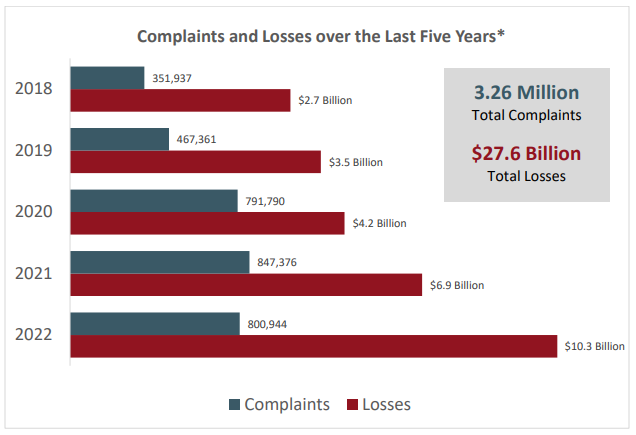
\includegraphics[width=350pt]{images/ic3_annual.png}
    \caption{FBI's 2022 Internet Crime Complaint Center (IC3) Annual Internet Crime Report}
    \label{fig:ice3_annual}
\end{figure}

\begin{verbatim}
\begin{figure}[h]
\centering
\includegraphics[width=0.5\textwidth]{image_file}
\caption{Caption of the image.}
\label{fig:my_label}
\end{figure}
\end{verbatim}

\subsection{Tables}
To add a table, you can use the table and tabular environments.

\begin{table}[ht]
\centering
\begin{tabular}{|c|c|}
\hline
Header 1 & Header 2 \\
\hline
Item 1   & Item 2   \\
\hline
\end{tabular}
\caption{Caption of the table.}
\label{tab:my_label}
\end{table}



\begin{verbatim}
\begin{table}[h]
\centering
\begin{tabular}{|c|c|}
\hline
Header 1 & Header 2 \\
\hline
Item 1   & Item 2   \\
\hline
\end{tabular}
\caption{Caption of the table.}
\label{tab:my_label}
\end{table}
\end{verbatim}

\subsection{Citing References}

References are an important part of any academic document. They not only acknowledge the work of others, but also allow readers to verify and follow-up your work. LaTeX makes citing references quite easy with the use of BibTeX, a tool for formatting lists of references.

BibTeX database files have a simple structure and they are easy to create. A `.bib` file is already included in this template in the `includes/` folder. An example of how to add a reference to this file is shown below:

\begin{verbatim}
@article{
    author = {John Doe},
    title = {Title of the Paper},
    year = {2020},
    journal = {Journal Name},
    volume = {4},
    pages = {10-20},
    publisher = {Publisher}
}
\end{verbatim}

Once your references are included in the `.bib` file, you can cite them in your text using the `\cite{}` command. The argument to the `\cite{}` command is the citation key, which is a unique identifier for each reference. In the example above, the citation key is `Doe2020`.

Here is an example of how to use the `\cite{}` command:

\begin{verbatim}
As stated by Doe \cite{Doe2020}, the usage of LaTeX simplifies document preparation.
\end{verbatim}

In the final document, this would appear as:

\begin{quote}
As stated by Doe [1], the usage of LaTeX simplifies document preparation.
\end{quote}


\subsection{Mathematical Expressions}
LaTeX is great for typesetting mathematical expressions. Enclose inline mathematical expressions with \$. For example, \verb|$E = mc^2$| will produce \(E = mc^2\). For numbered equations on their own lines, use the equation environment.

\begin{verbatim}
\begin{equation}
a^2 + b^2 = c^2
\label{eq:pythagorean}
\end{equation}
\end{verbatim}

\subsection{Page Breaks}
You can force a page break using the \verb|\clearpage| command. This is particularly useful when you want to control where new content starts.

\begin{verbatim}
\clearpage
\end{verbatim}

\subsection{Vertical Spacing}
You can control vertical spacing using the \verb|\vspace{length}| command. The length can be specified in various units, such as pt (points), mm (millimeters), cm (centimeters), in (inches), em (the width of the letter M in the current font), and ex (the height of the letter x in the current font).

\begin{verbatim}
\vspace{1cm}
This line is 1 cm below the previous line.
\end{verbatim}

\subsection{Horizontal Spacing}
For horizontal spacing, use the \verb|\hspace{length}| command. The length units are the same as for \verb|\vspace|.

\begin{verbatim}
This is \hspace{2cm} two cm space.
\end{verbatim}

\subsection{New Paragraphs and Line Breaks}
To start a new paragraph, leave a blank line in your LaTeX code. To force a line break without starting a new paragraph, use the \verb|\\| command.

\begin{verbatim}
This is a paragraph.

This is another paragraph.\\
This is a new line in the same paragraph.
\end{verbatim}

Remember that LaTeX is designed to provide excellent typography and layout out of the box, so manual spacing and page breaks should generally be used sparingly.

\chapter{Literature Review}

\section*{Guidelines for Literature Review}
The Literature Review chapter should provide a detailed review of the current literature related to your research topic. 

This is an important part of your paper, and it's usually substantial, typically around 15-20 pages or approximately 4500-6000 words. 

Here are some points you may want to consider:
\begin{itemize}
    \item Your review should summarize and synthesize the relevant literature on your topic.
    \item It should evaluate the sources and advise the reader on the most pertinent or relevant.
    \item It should demonstrate your familiarity with the topic and how your proposed research fits within the larger field of study.
    \item The literature review should be organized thematically, not by source. This means you should group research studies or other types of literature (reports, articles, etc.) together by common themes or points, not by the authors or the publications.
\end{itemize}

\section{Subsection1}
%Discussion of the first topic

\section{Subsection2}
%Discussion of the second topic

%Continue with further subsections as required

\section{Summary}
%Summary of the main findings of your literature review

\chapter{Your Chapters}


\chapter{Results}

\section*{Guidelines for Results}
The Results chapter presents your findings in detail, referring to the graphs, tables, or other means of data representation you have included. 

This chapter is typically around 10-15 pages or approximately 3000-4500 words. However, the length can vary depending on the quantity and complexity of the data to be presented.

Here are some points you may want to consider:
\begin{itemize}
    \item Results should be clearly and concisely presented. Avoid unnecessary verbosity.
    \item Use graphs, charts, tables, and other visual aids as needed to display your data. These should be clearly labelled, properly referenced and discussed in the text.
    \item Do not include analysis or interpretation of the results in this section. This will be done in the Discussion chapter.
    \item Make sure to present all of your relevant results, including those that do not support your hypothesis or unexpected results. 
\end{itemize}


\section{Subsection1}
%Discussion of the first set of results

\section{Subsection2}
%Discussion of the second set of results

\chapter{Discussion}

\section*{Guidelines for Discussion Section}
In the discussion section, you should interpret and elaborate on your results or findings, drawn from the data you have collected and the analysis performed. 

This is one of the most substantial sections of your paper, so it could span several pages (typically 4-5 pages or around 2000-3000 words in a long document such as a thesis). 

Here are some points you may want to consider:
\begin{itemize}
    \item Relate your findings to the objectives of the study.
    \item Explain how your results relate to the expectations and to the literature cited in your Literature Review.
    \item Discuss any unexpected findings.
    \item Describe why you think certain outcomes occurred and what led you to these conclusions.
    \item Discuss the broader implications of those outcomes.
    \item You may also propose areas for further research.
\end{itemize}


\chapter{Conclusion}

\section*{Guidelines for Conclusion Section}
The conclusion section provides a succinct summary of your findings and implications. This is usually a shorter section, generally about 1-2 pages or around 500-1000 words in a long document such as a thesis. 

Here are some points you may want to consider:
\begin{itemize}
    \item Summarize the main points from the body of your paper, including the major findings, and the key arguments or discoveries. This should be done briefly and be linked back to the aim and objectives of your study.
    \item Discuss the broader impact of your results. How does your research contribute to your field of study? 
    \item Describe the limitations of your study. No study is perfect, and acknowledging the weaknesses or gaps in your research honestly could make your conclusions more persuasive.
    \item Suggest areas for future research. Are there aspects that you couldn't cover fully or ideas that would be beneficial to explore in the future?
\end{itemize}

% Bibliography
\bibliographystyle{ieeetr} % Use IEEE Transactions bibliography style
\bibliography{includes/references} % Reference list located in 'includes/references.bib'

\end{document}
